% Chapter 2: Exploratory Data Analysis
\chapter{Exploratory Data Analysis}

\section{Data Overview}
\subsection{Dataset Structure}
The Ames Housing dataset comprises residential property sales in Ames, Iowa from 2006 to 2010. The dataset contains:
\begin{itemize}
    \item 1,460 observations in the training set
    \item 79 explanatory variables (23 nominal, 23 ordinal, 14 discrete, and 20 continuous)
    \item Target variable: Sale Price (continuous)
\end{itemize}

\subsection{Variable Categories}
The variables can be grouped into several categories:
\begin{itemize}
    \item Location-related features (e.g., Neighborhood, Condition)
    \item Building characteristics (e.g., Overall Quality, Year Built)
    \item Room information (e.g., Total Rooms, Bedrooms)
    \item Size measurements (e.g., Total Living Area, Lot Area)
    \item Quality and condition ratings
    \item Sale conditions and types
\end{itemize}

\section{Missing Value Analysis}
\begin{figure}[H]
    \centering
    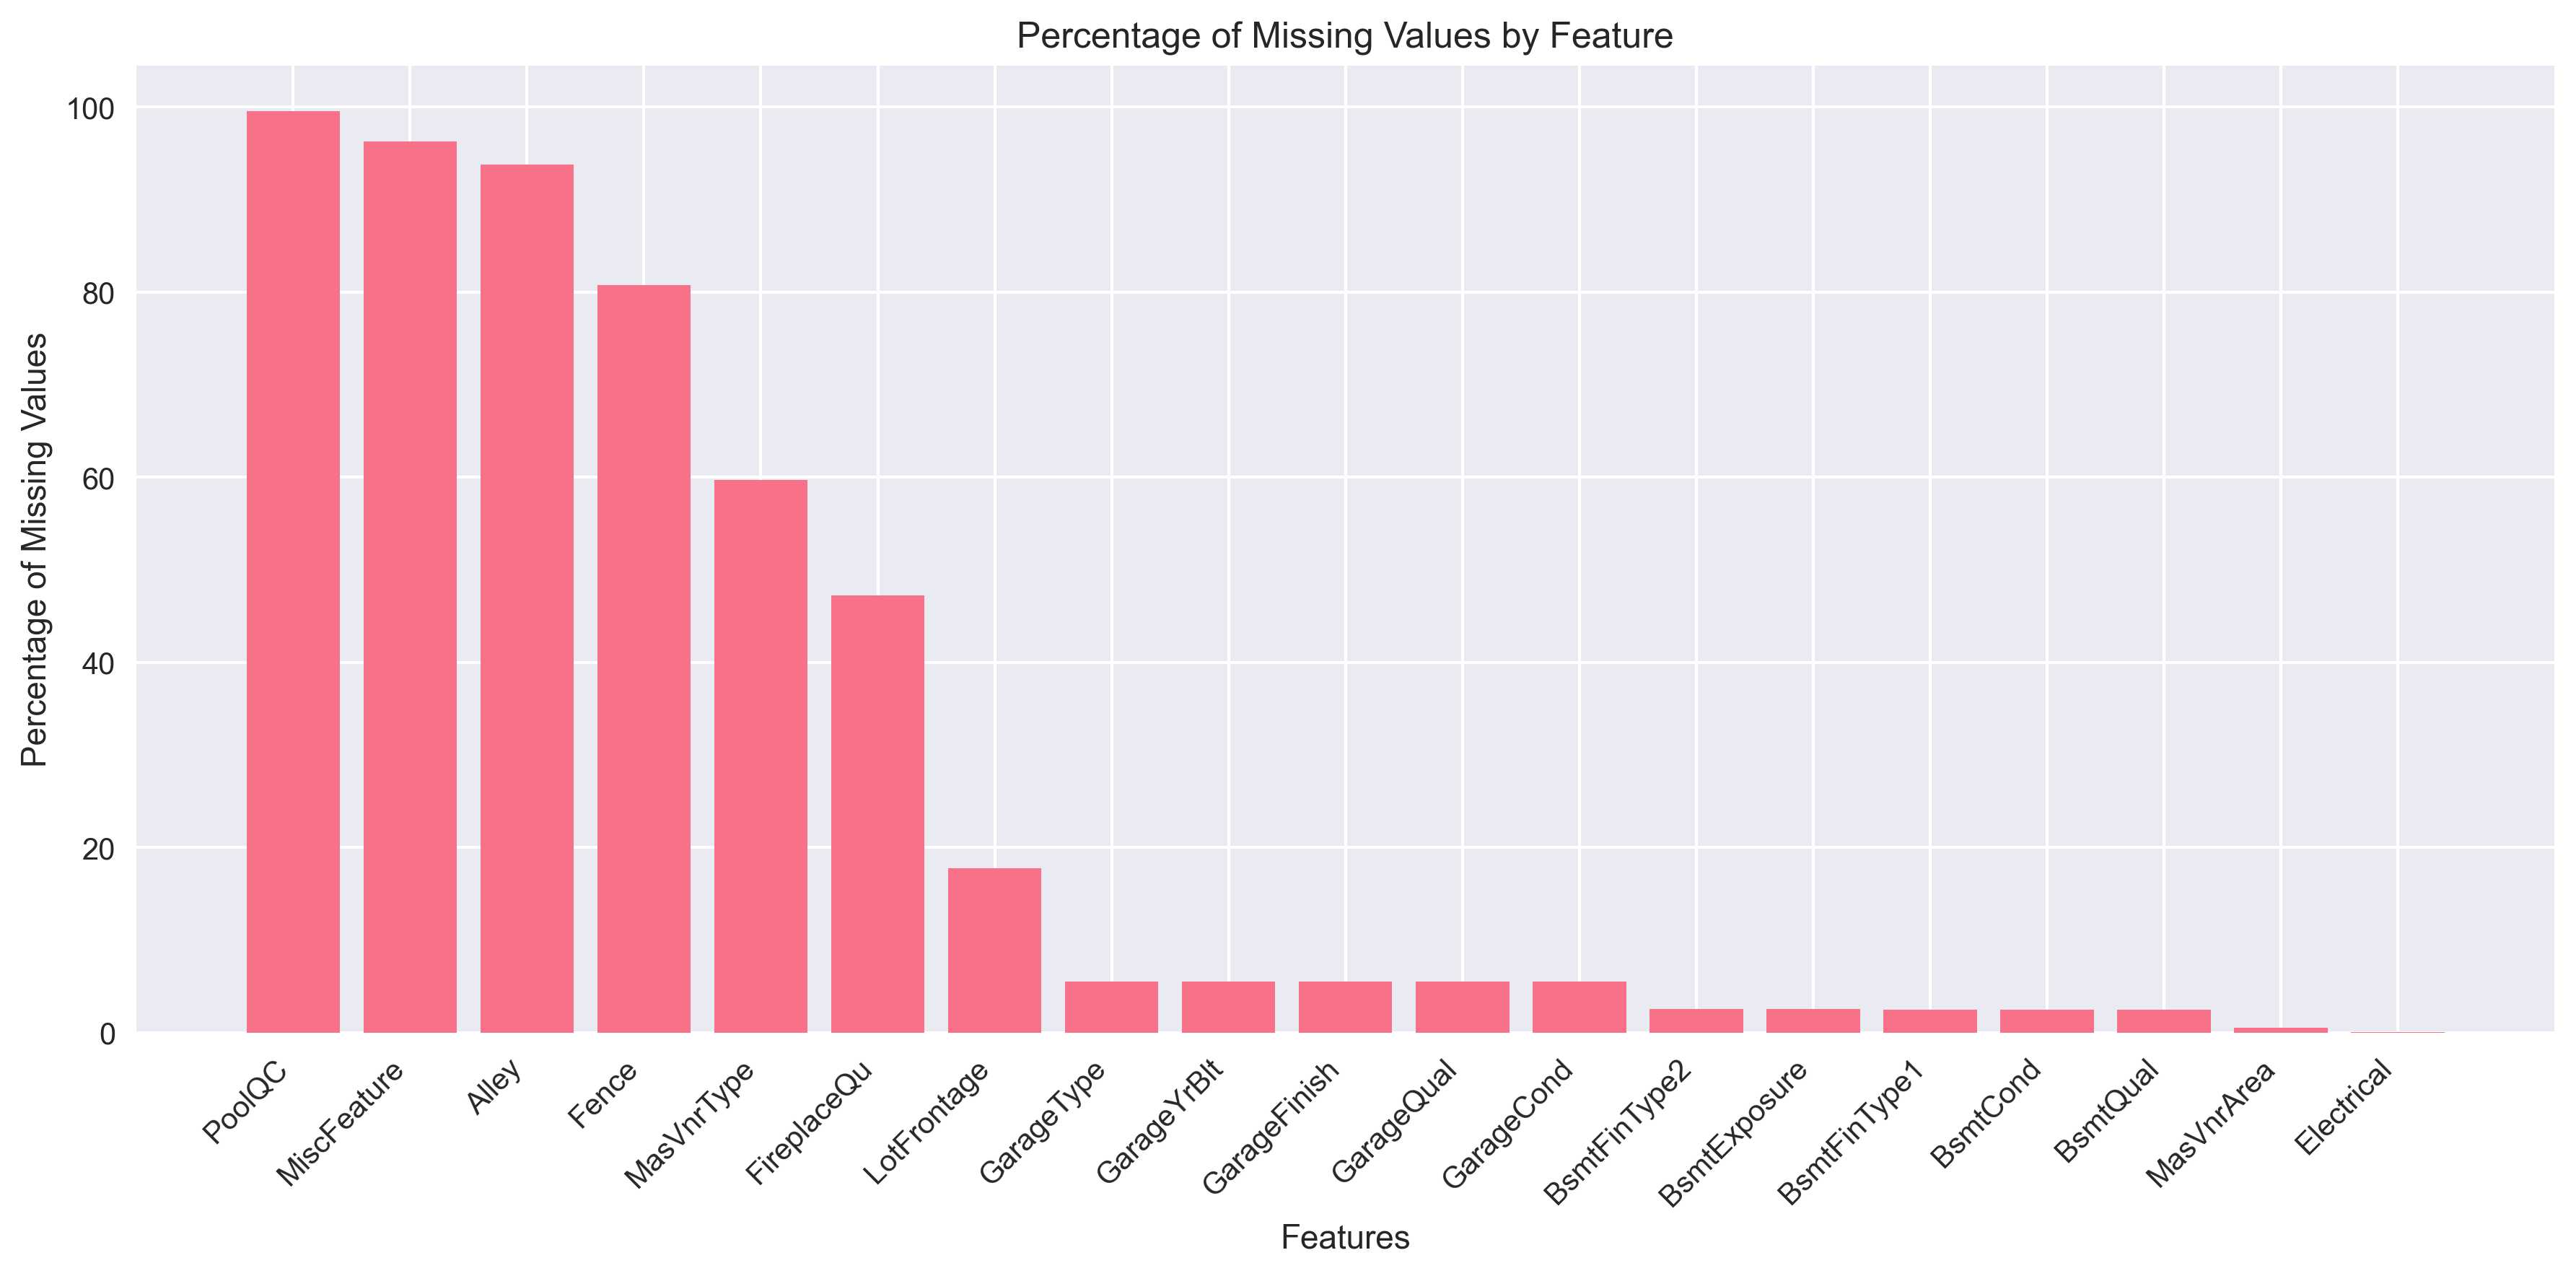
\includegraphics[width=1.0\textwidth]{figures/missing_values.png}
    \caption{Distribution of Missing Values Across Features}
    \label{fig:missing_values}
\end{figure}

The analysis of missing values reveals several patterns:
\begin{itemize}
    \item Pool QC has the highest percentage of missing values (99.5\%), which is expected as most houses in Iowa don't have pools
    \item Features like Alley (93.8\% missing) and Fence (80.7\% missing) are also frequently missing, indicating these are optional features
    \item Most missing values appear in categorical variables describing specific features that may not be present in all houses
    \item For modeling purposes, missing values in categorical variables will be treated as 'None' or 'Not Available'
\end{itemize}

\section{Target Variable Analysis}
\begin{figure}[H]
    \centering
    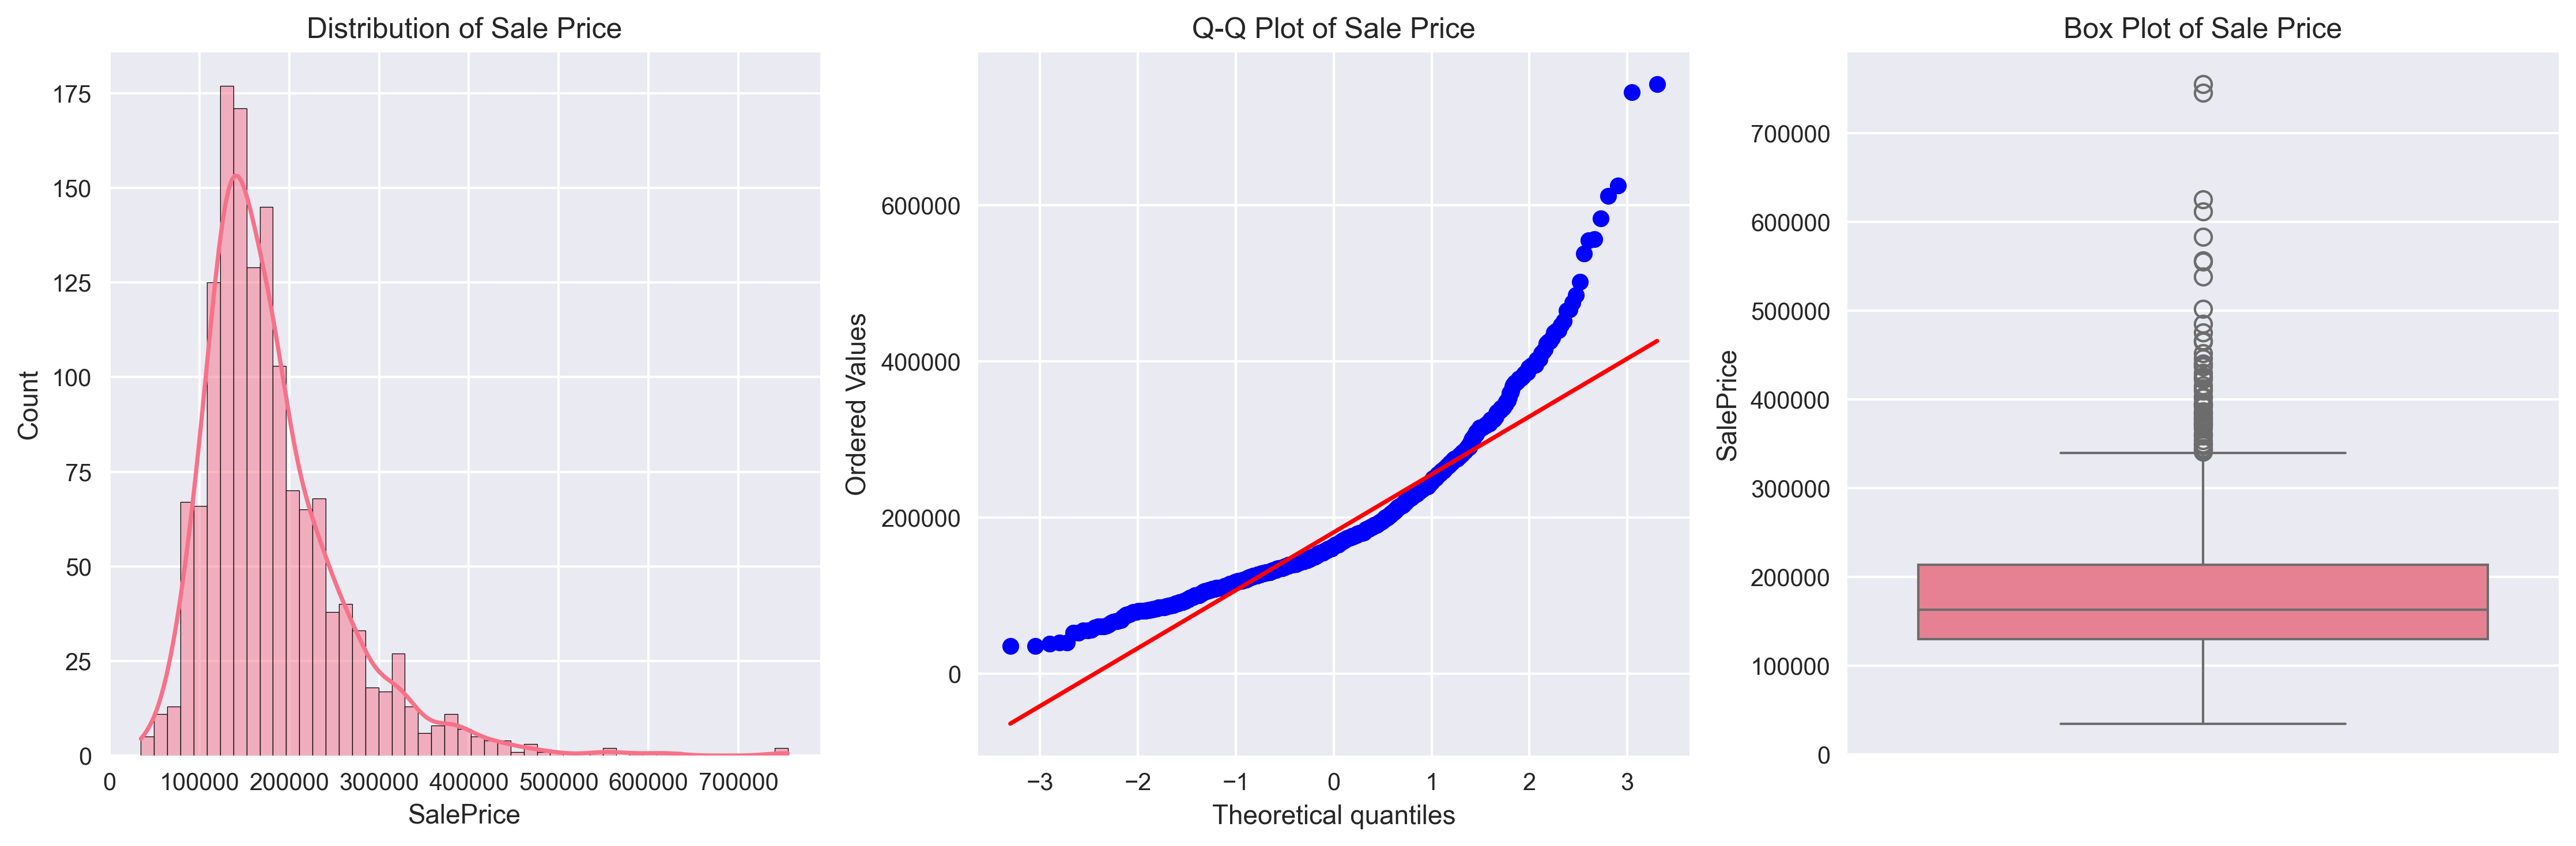
\includegraphics[width=1.0\textwidth]{figures/sale_price_distribution.png}
    \caption{Distribution and Statistical Properties of Sale Price}
    \label{fig:sale_price_dist}
\end{figure}

The sale price distribution exhibits several key characteristics:
\begin{itemize}
    \item Right-skewed distribution with a mean of \$180,921 and median of \$163,000
    \item Significant positive skewness (1.88) indicating more lower-priced homes
    \item Presence of high-value outliers above \$400,000
    \item Q-Q plot shows deviation from normality, suggesting log transformation for modeling
    \item Price range spans from \$34,900 to \$755,000, showing wide market diversity
\end{itemize}

\section{Feature Analysis}
\subsection{Numerical Features}
\begin{figure}[H]
    \centering
    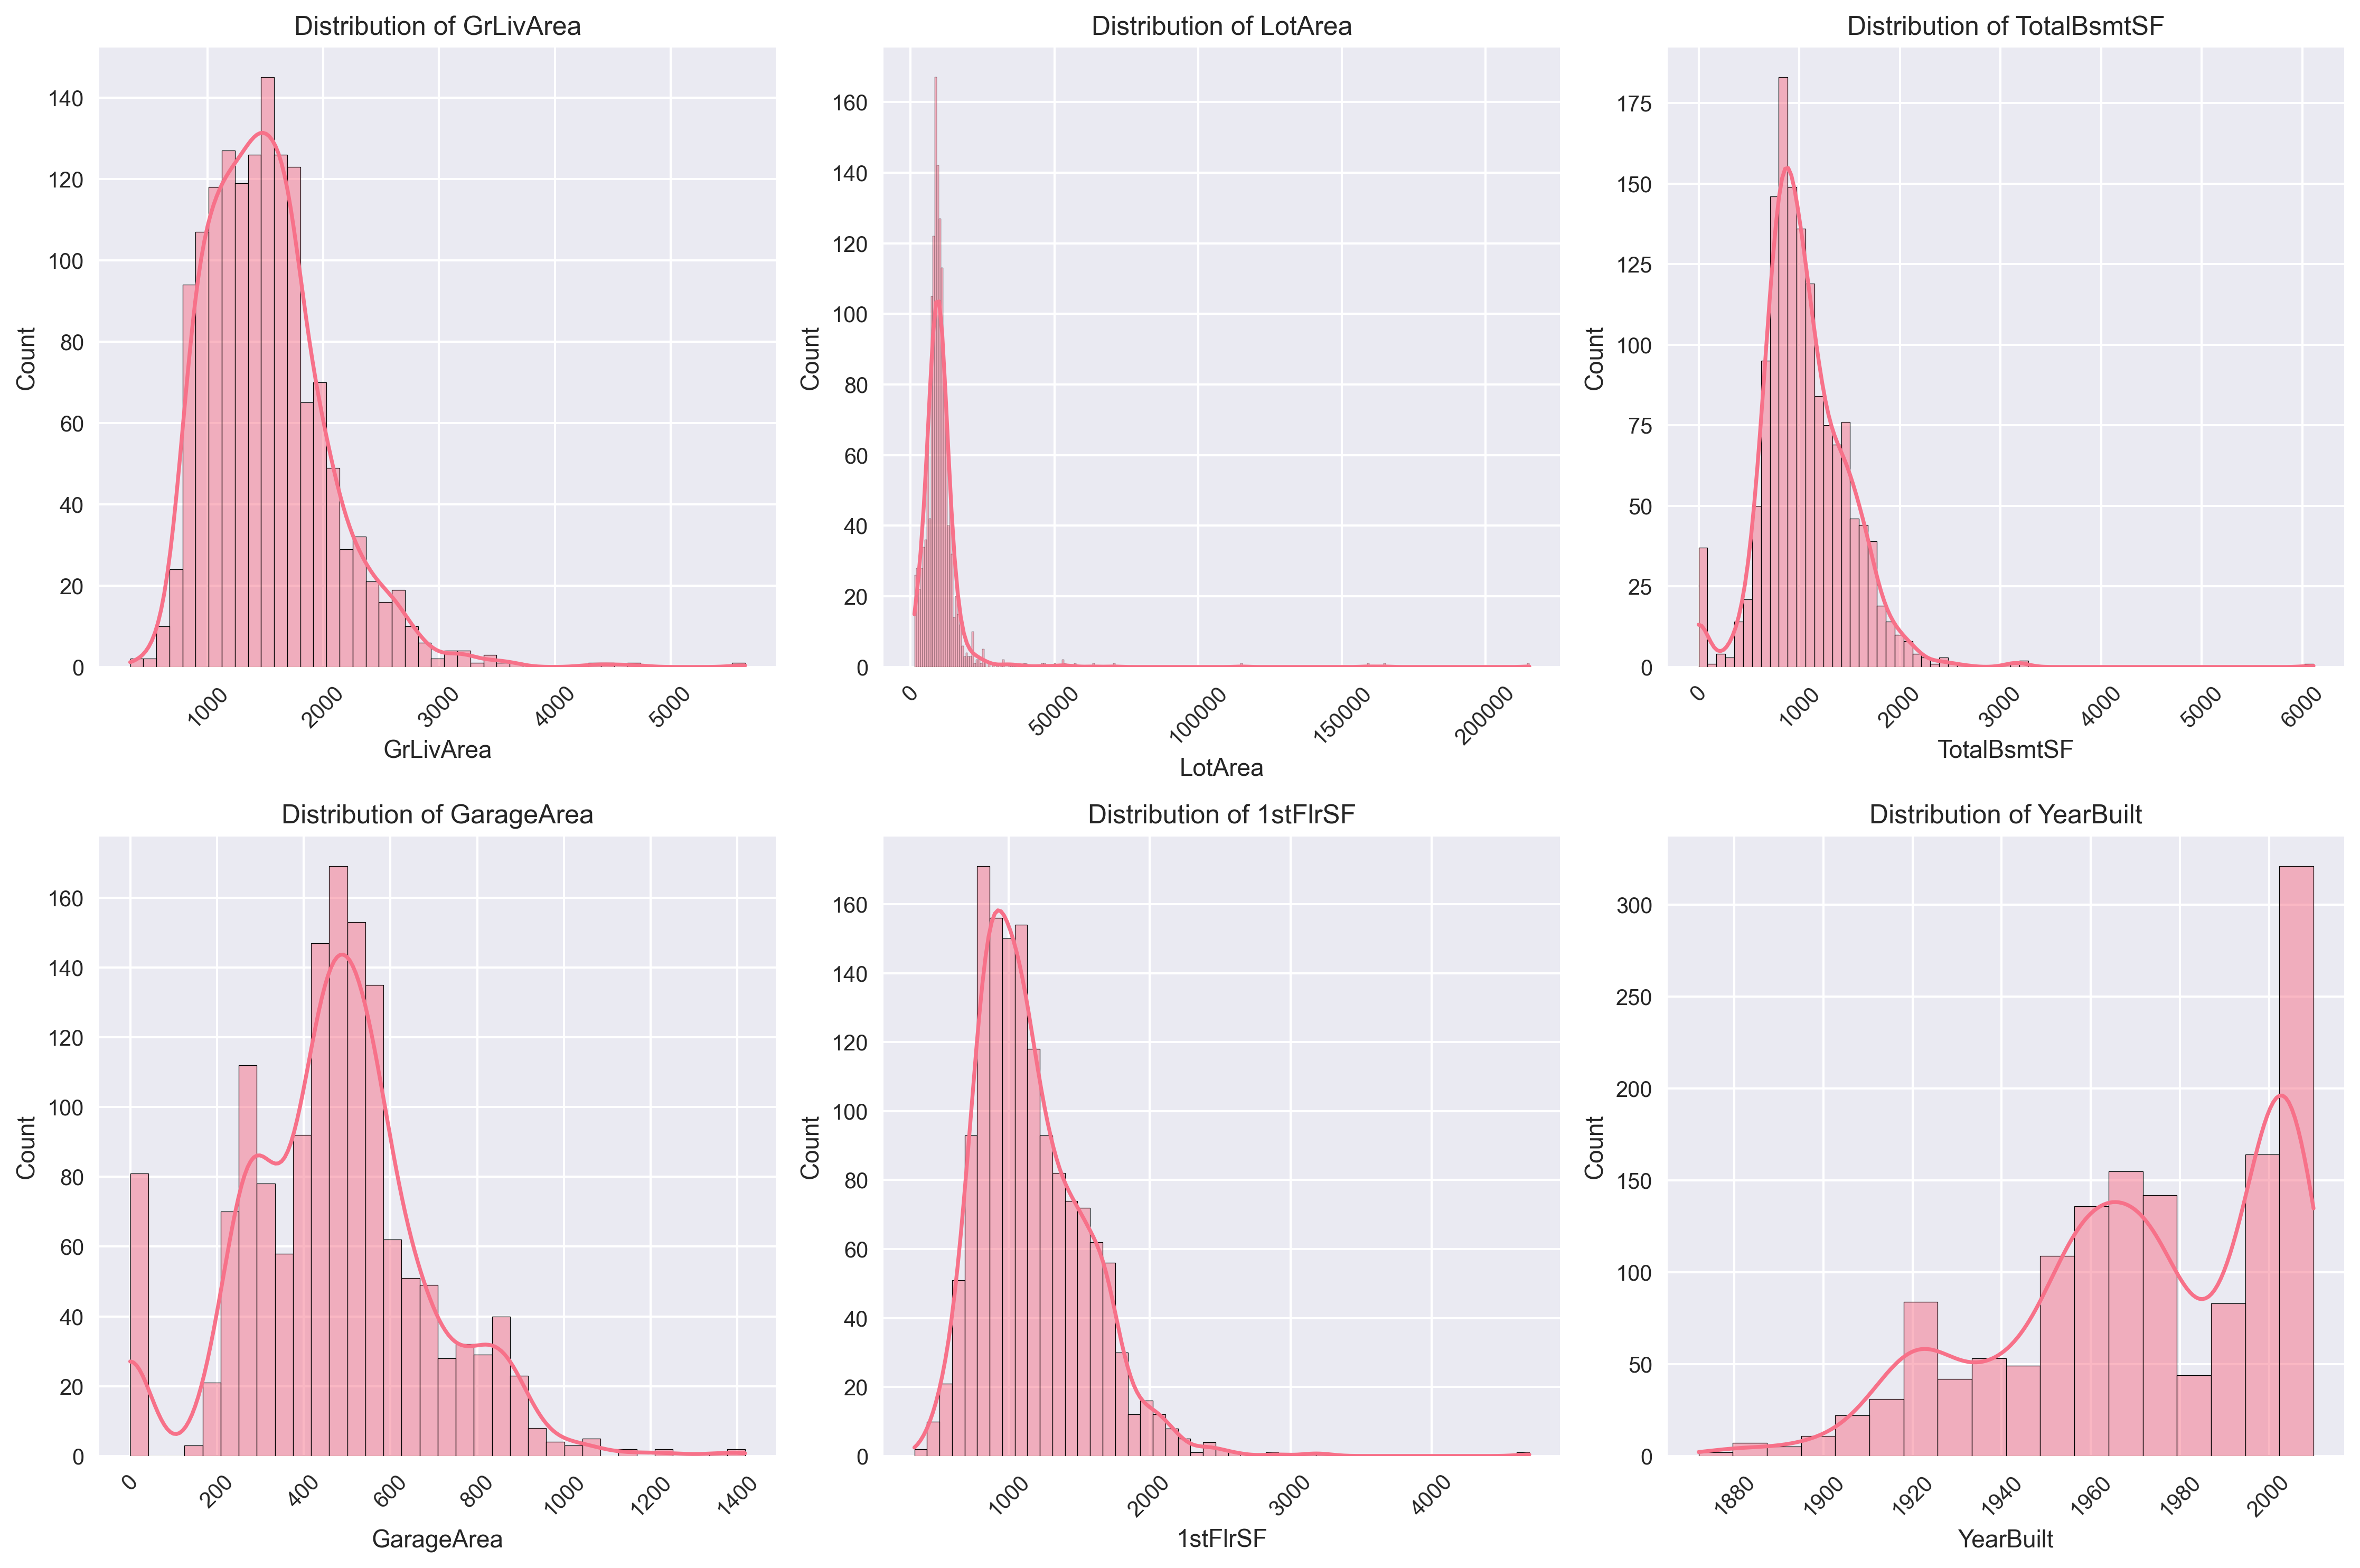
\includegraphics[width=1.0\textwidth]{figures/numerical_features_dist.png}
    \caption{Distribution of Key Numerical Features}
    \label{fig:num_features_dist}
\end{figure}

Key observations from numerical features:
\begin{itemize}
    \item Ground Living Area (GrLivArea) shows right-skewed distribution with most homes between 800-2000 sq ft
    \item Lot Area exhibits extreme right skew with several outliers, suggesting some very large properties
    \item Year Built shows multiple peaks, corresponding to different development periods in Ames
    \item Garage and Basement areas show similar patterns, with most homes having these features
\end{itemize}

\subsection{Feature Correlations}
\begin{figure}[H]
    \centering
    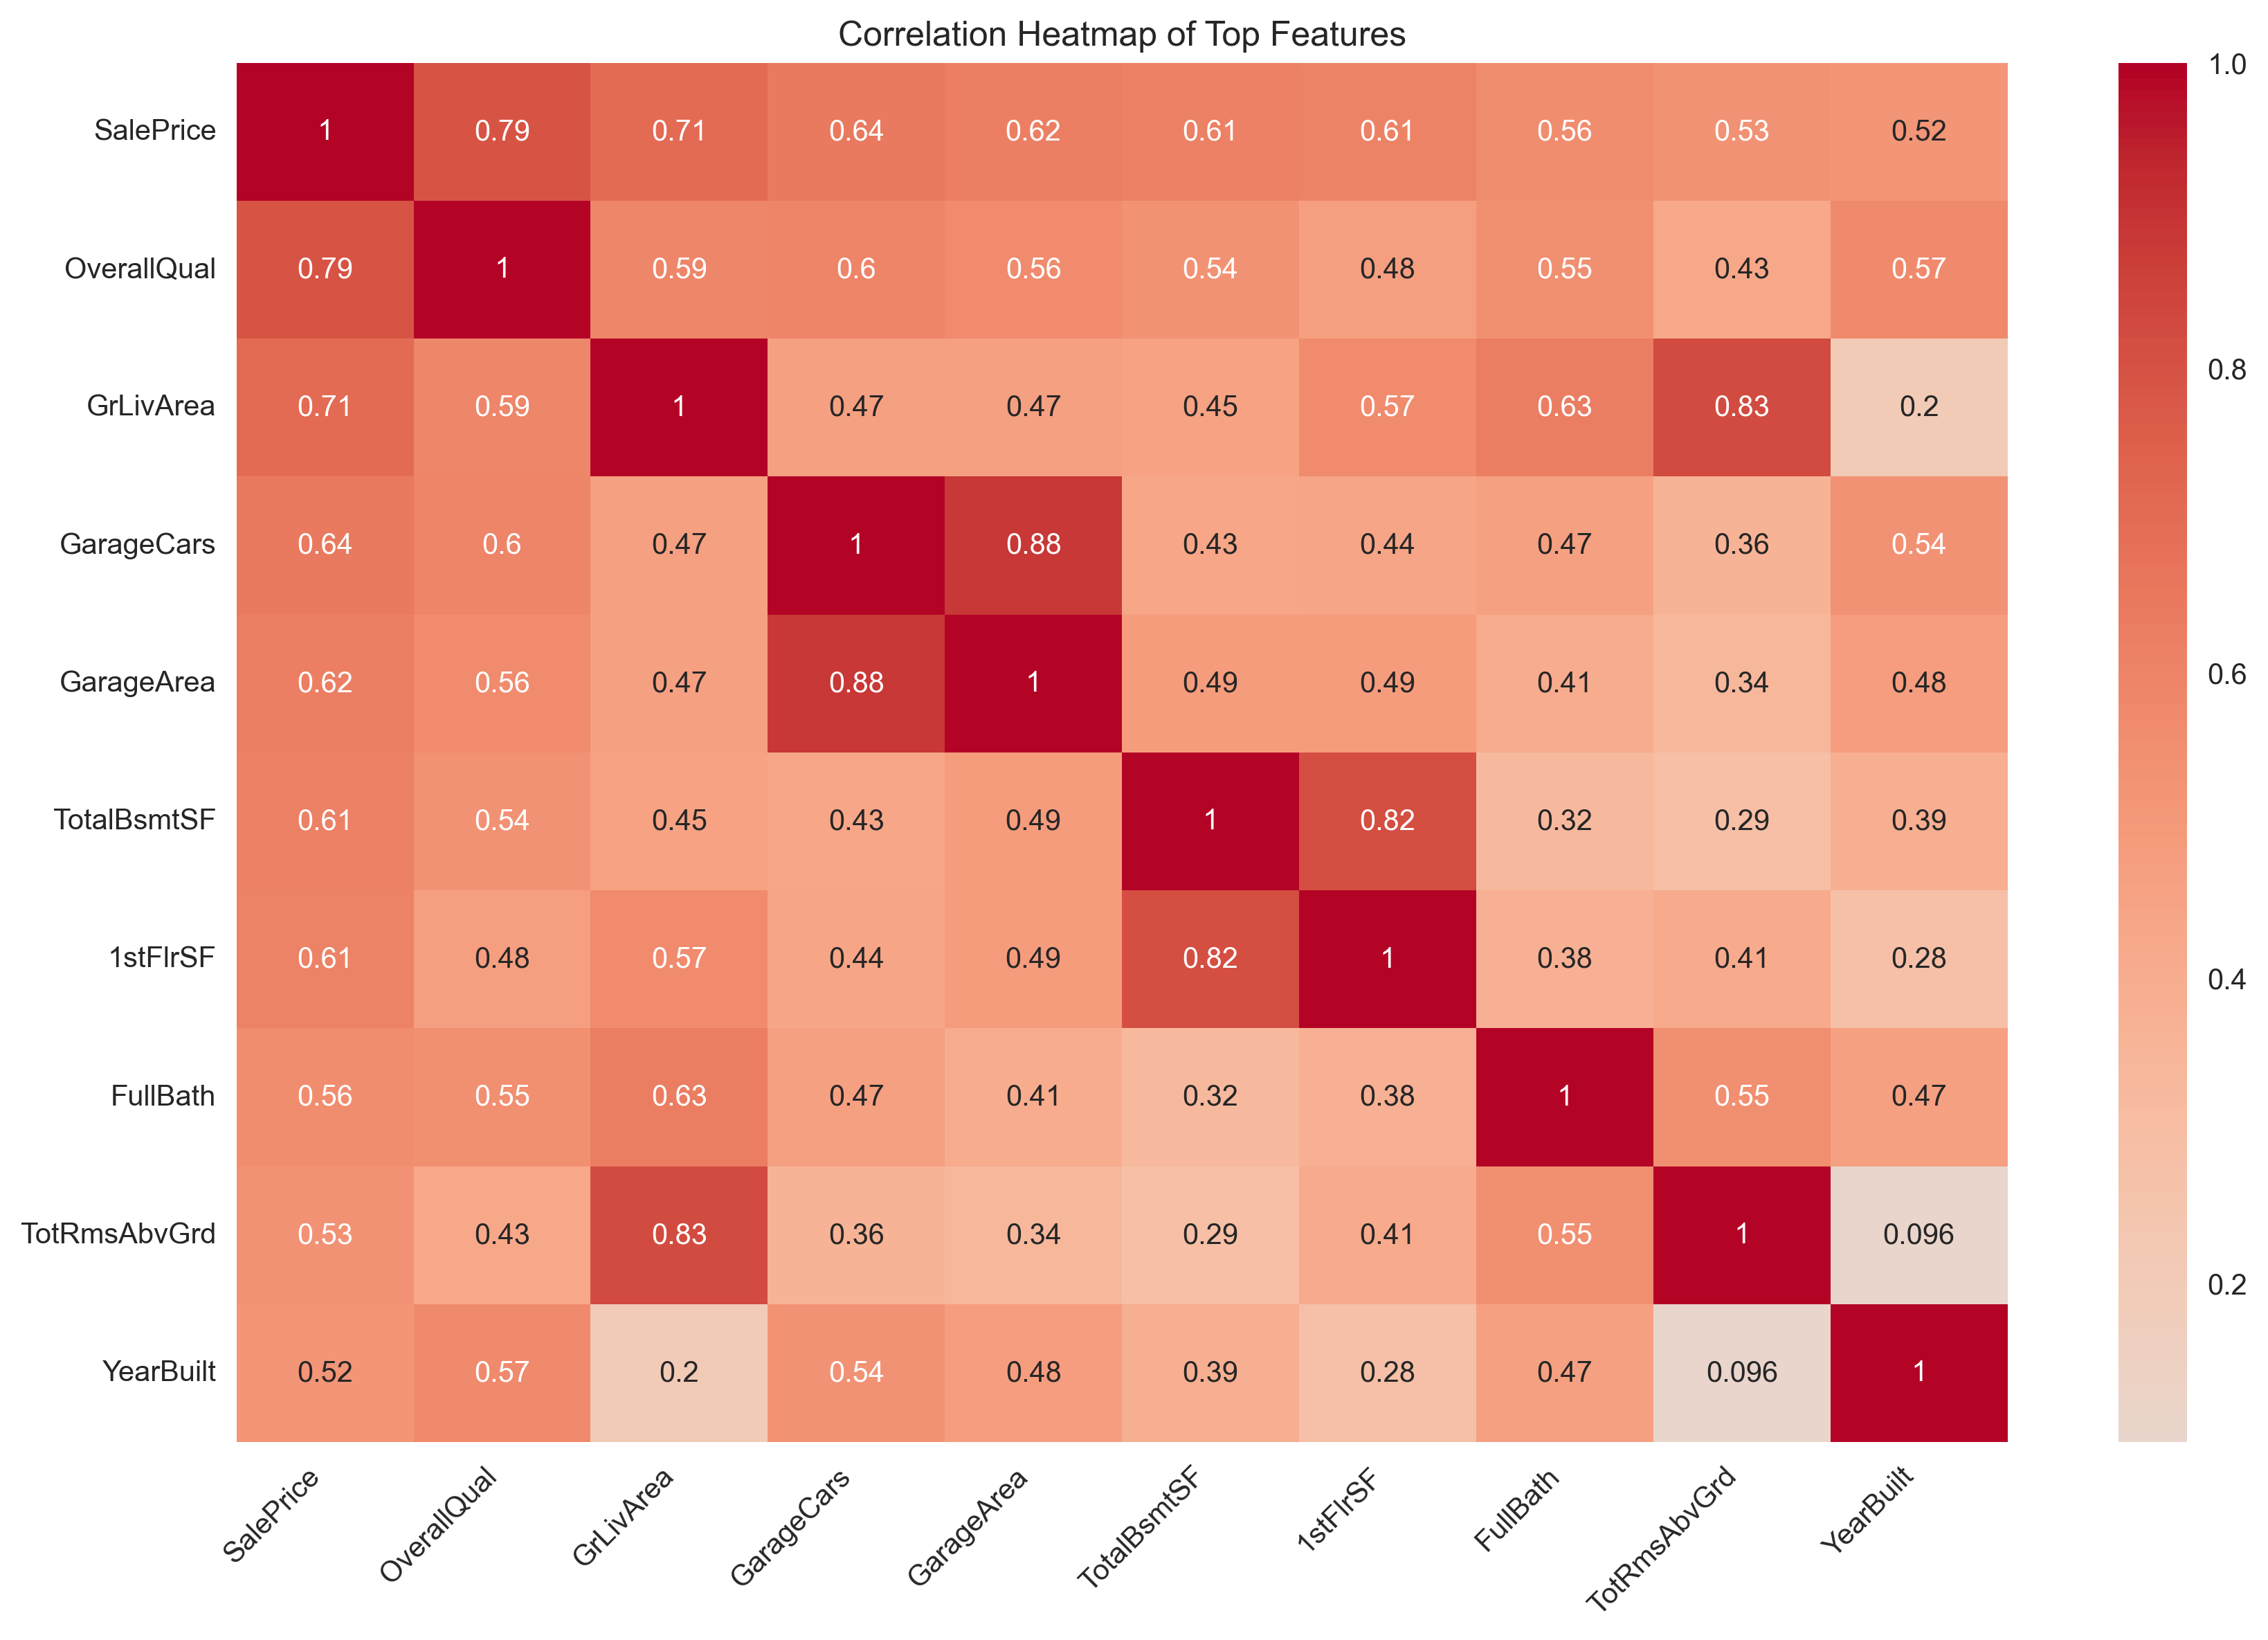
\includegraphics[width=1.0\textwidth]{figures/correlation_matrix.png}
    \caption{Correlation Matrix of Top Features}
    \label{fig:correlation_matrix}
\end{figure}

The correlation analysis reveals:
\begin{itemize}
    \item Overall Quality has the strongest correlation with Sale Price (0.79)
    \item Above Ground Living Area shows strong positive correlation (0.71)
    \item Garage Area and Total Basement SF have moderate correlations (0.62 and 0.61)
    \item Several features show multicollinearity, requiring careful feature selection
\end{itemize}

\subsection{Feature Relationships}
\begin{figure}[H]
    \centering
    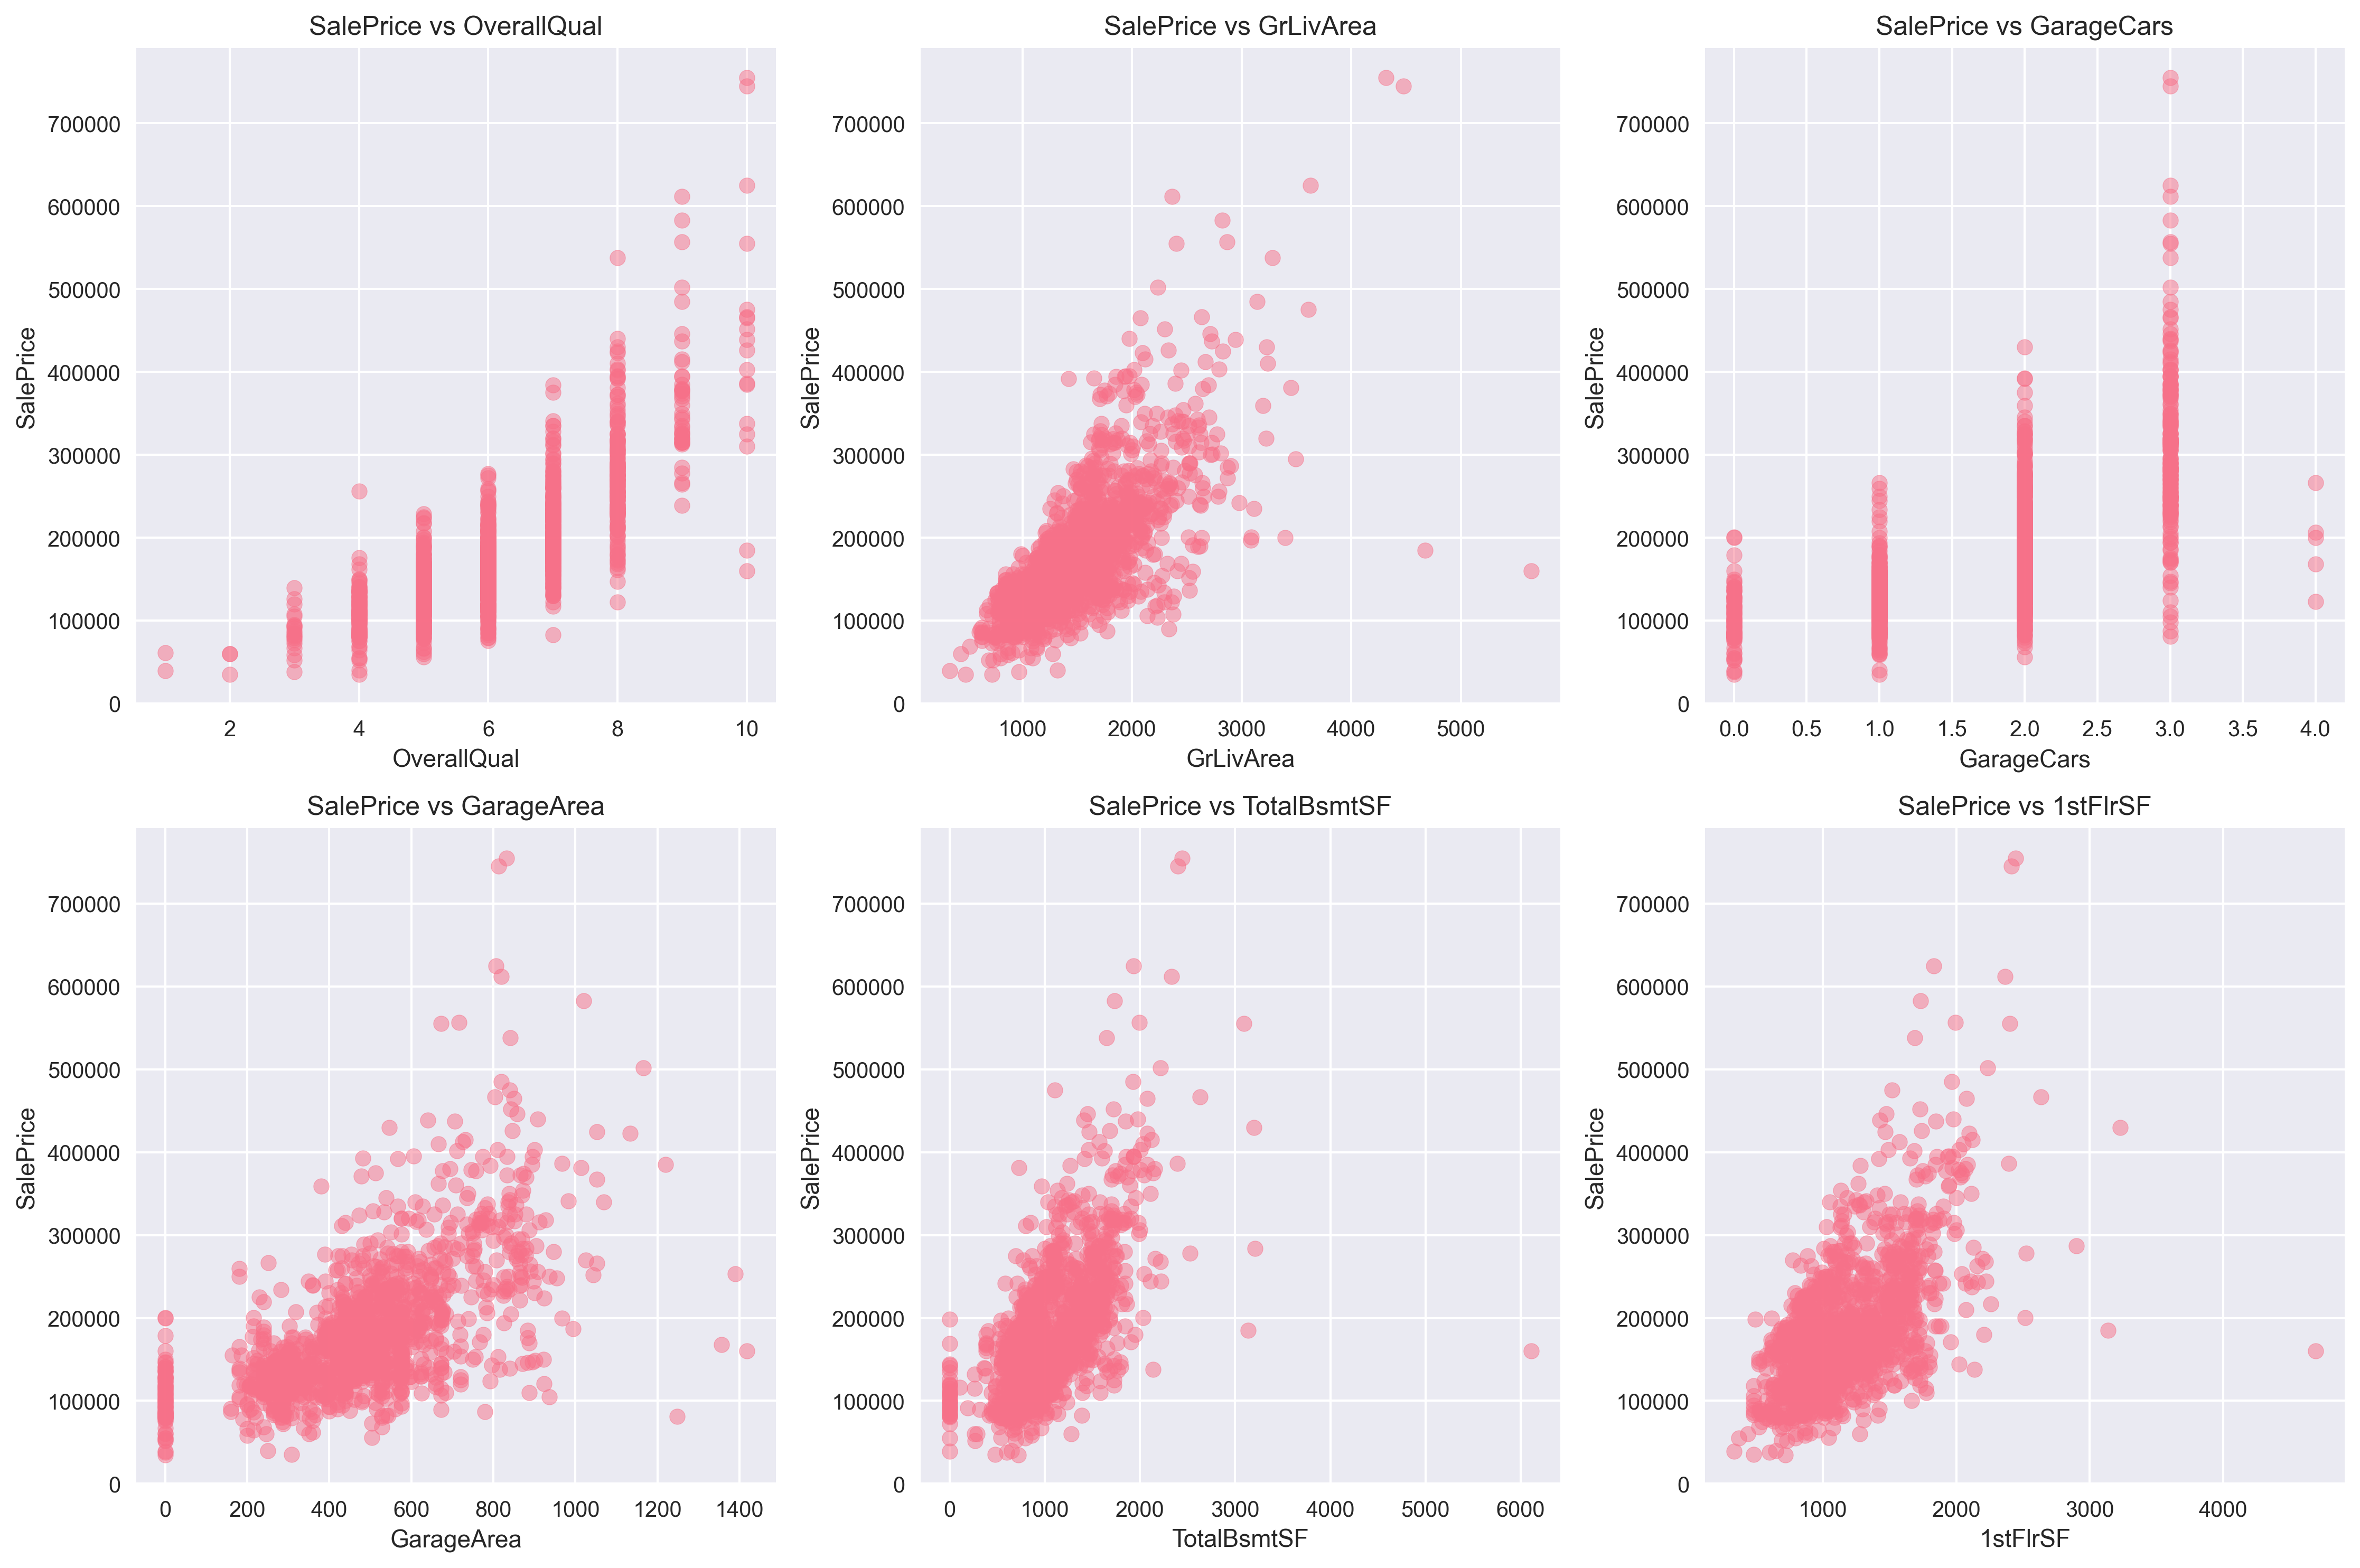
\includegraphics[width=1.0\textwidth]{figures/feature_vs_price.png}
    \caption{Relationships between Key Features and Sale Price}
    \label{fig:feature_price_relation}
\end{figure}

Analysis of feature relationships shows:
\begin{itemize}
    \item Strong linear relationship between Living Area and Price
    \item Overall Quality shows clear step-wise increase in price
    \item Garage Area shows positive correlation but with more scatter
    \item Year Built shows upward trend with newer homes commanding higher prices
\end{itemize}

\section{Categorical Features}
\begin{figure}[H]
    \centering
    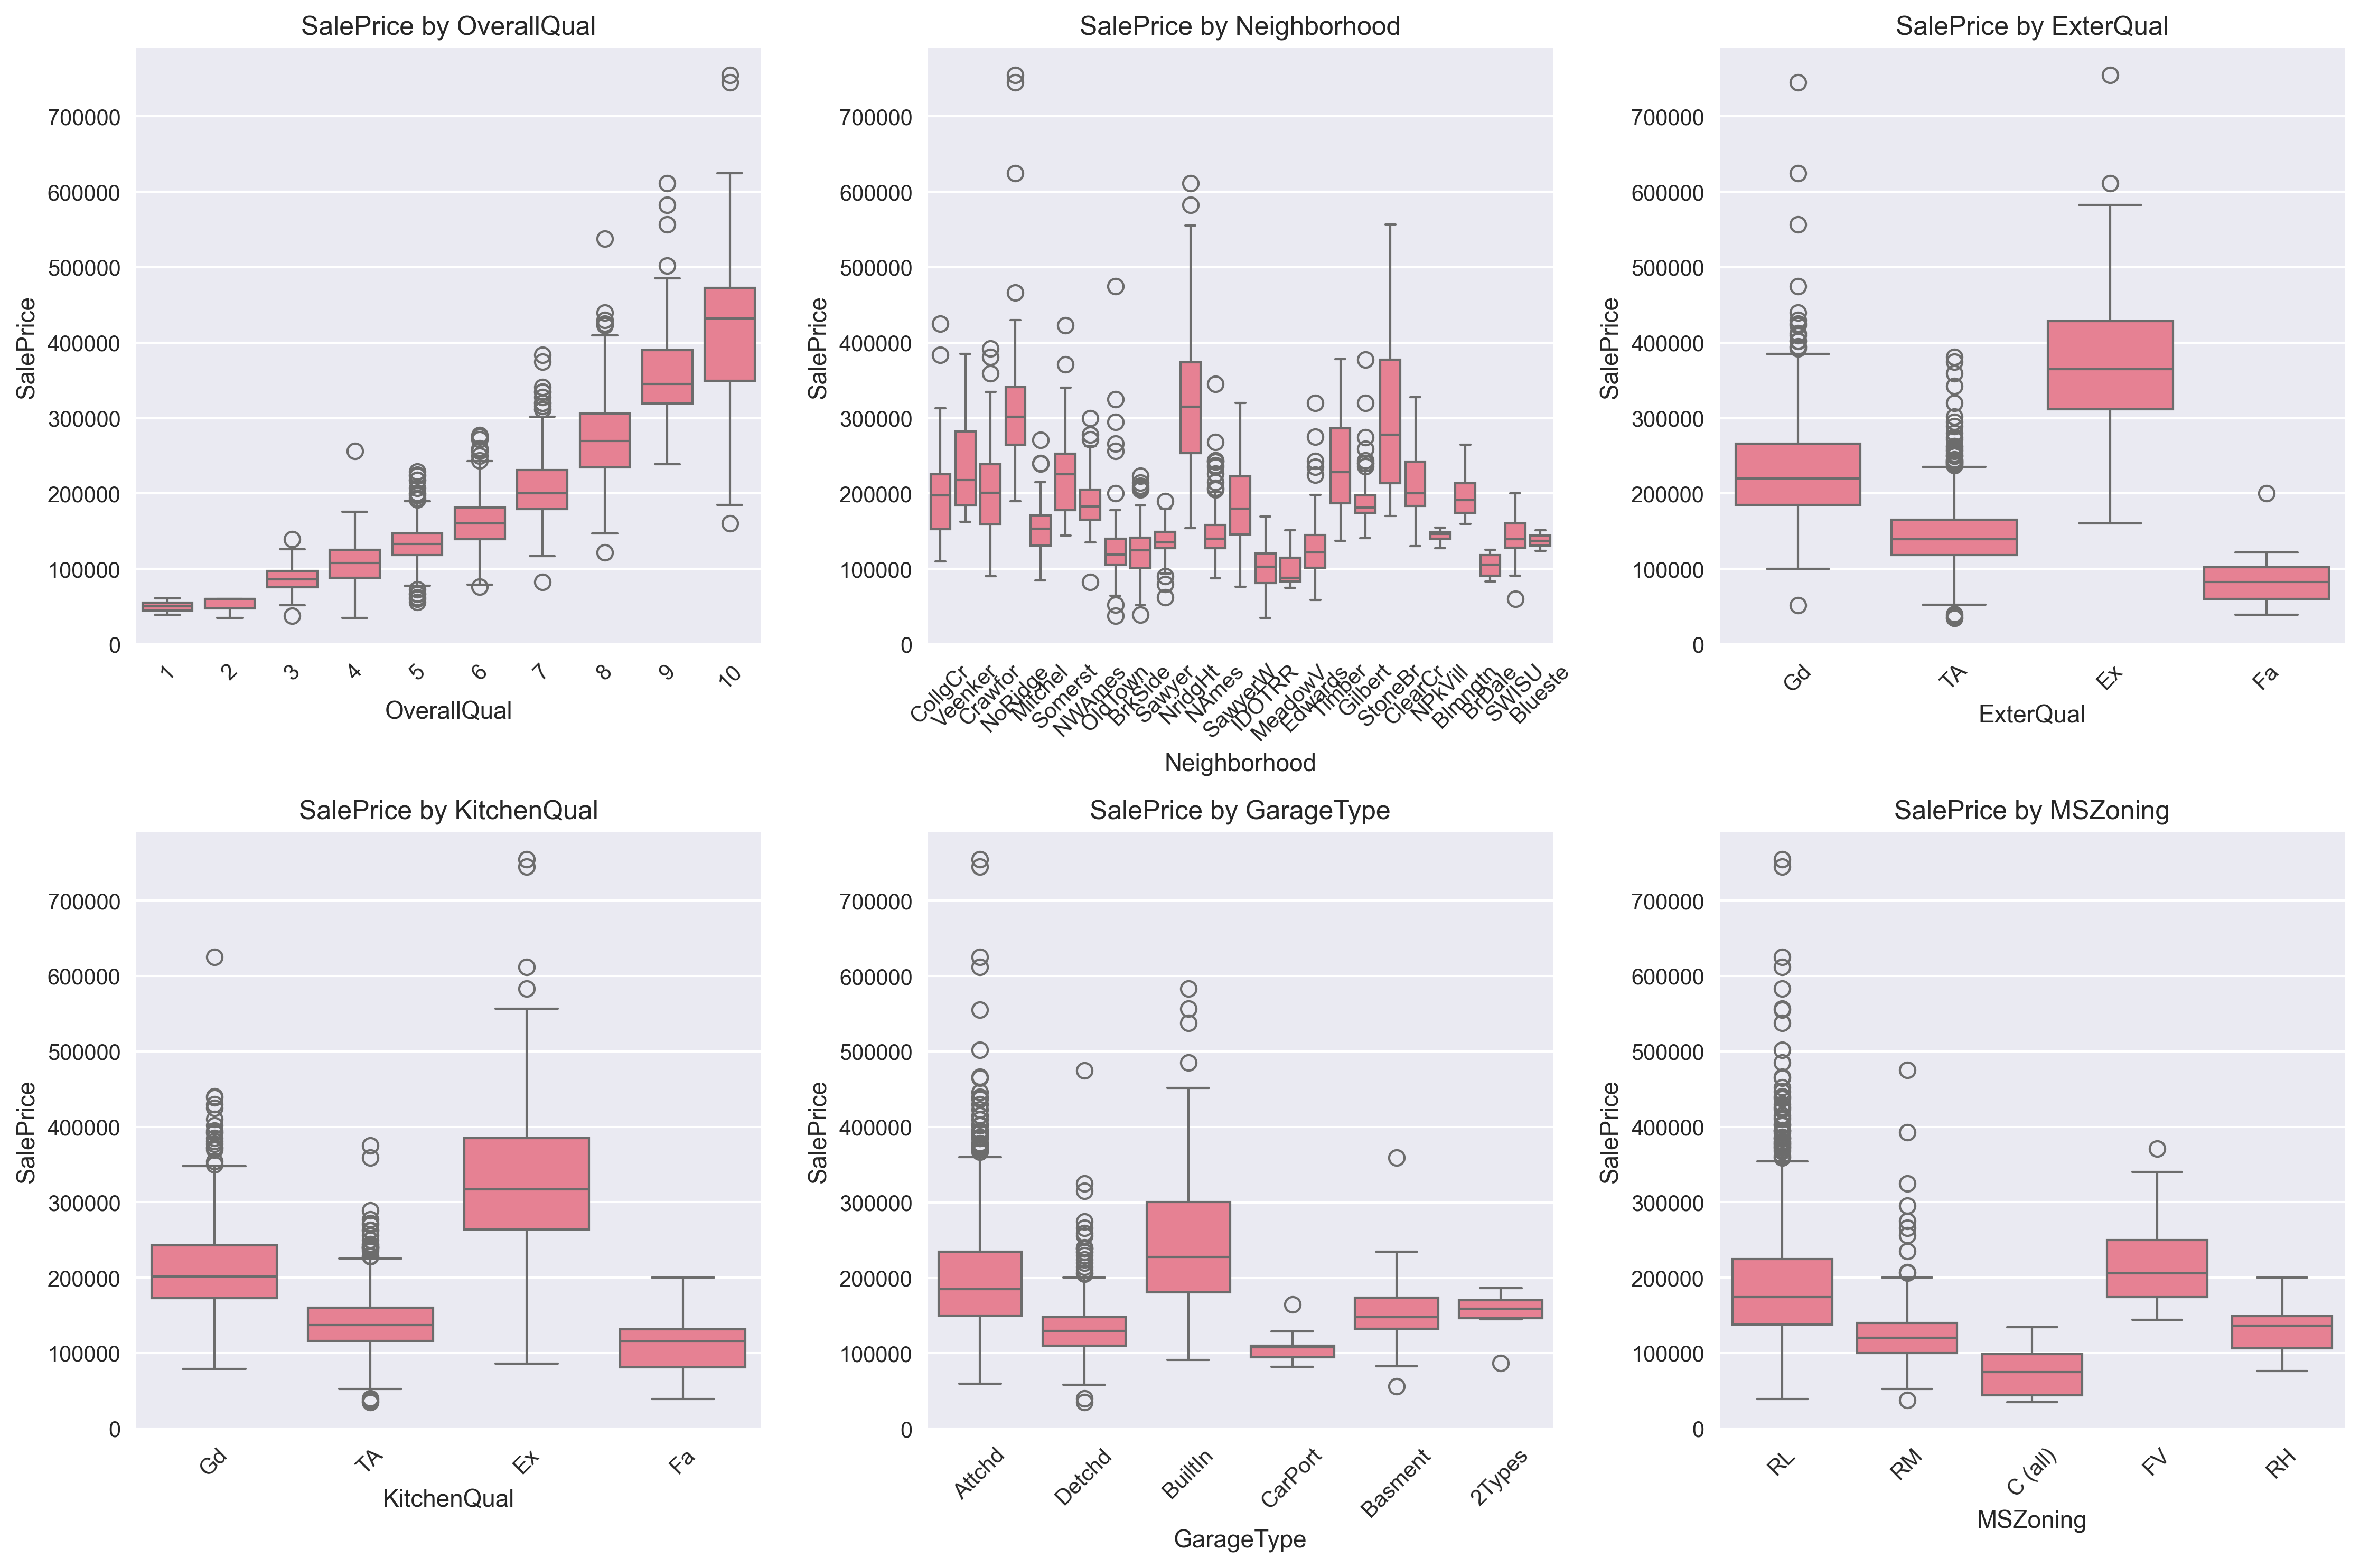
\includegraphics[width=1.0\textwidth]{figures/categorical_features_dist.png}
    \caption{Sale Price Distribution by Categorical Features}
    \label{fig:cat_features_dist}
\end{figure}

Important findings from categorical analysis:
\begin{itemize}
    \item Neighborhood significantly influences price, with NoRidge and NridgHt commanding highest prices
    \item Overall Quality shows clear price progression from 1 to 10
    \item Kitchen and Exterior Quality ratings strongly correlate with price
    \item Zoning categories show distinct price ranges, with RL (Residential Low Density) being most common
\end{itemize}

\section{Outlier Analysis}
\begin{figure}[H]
    \centering
    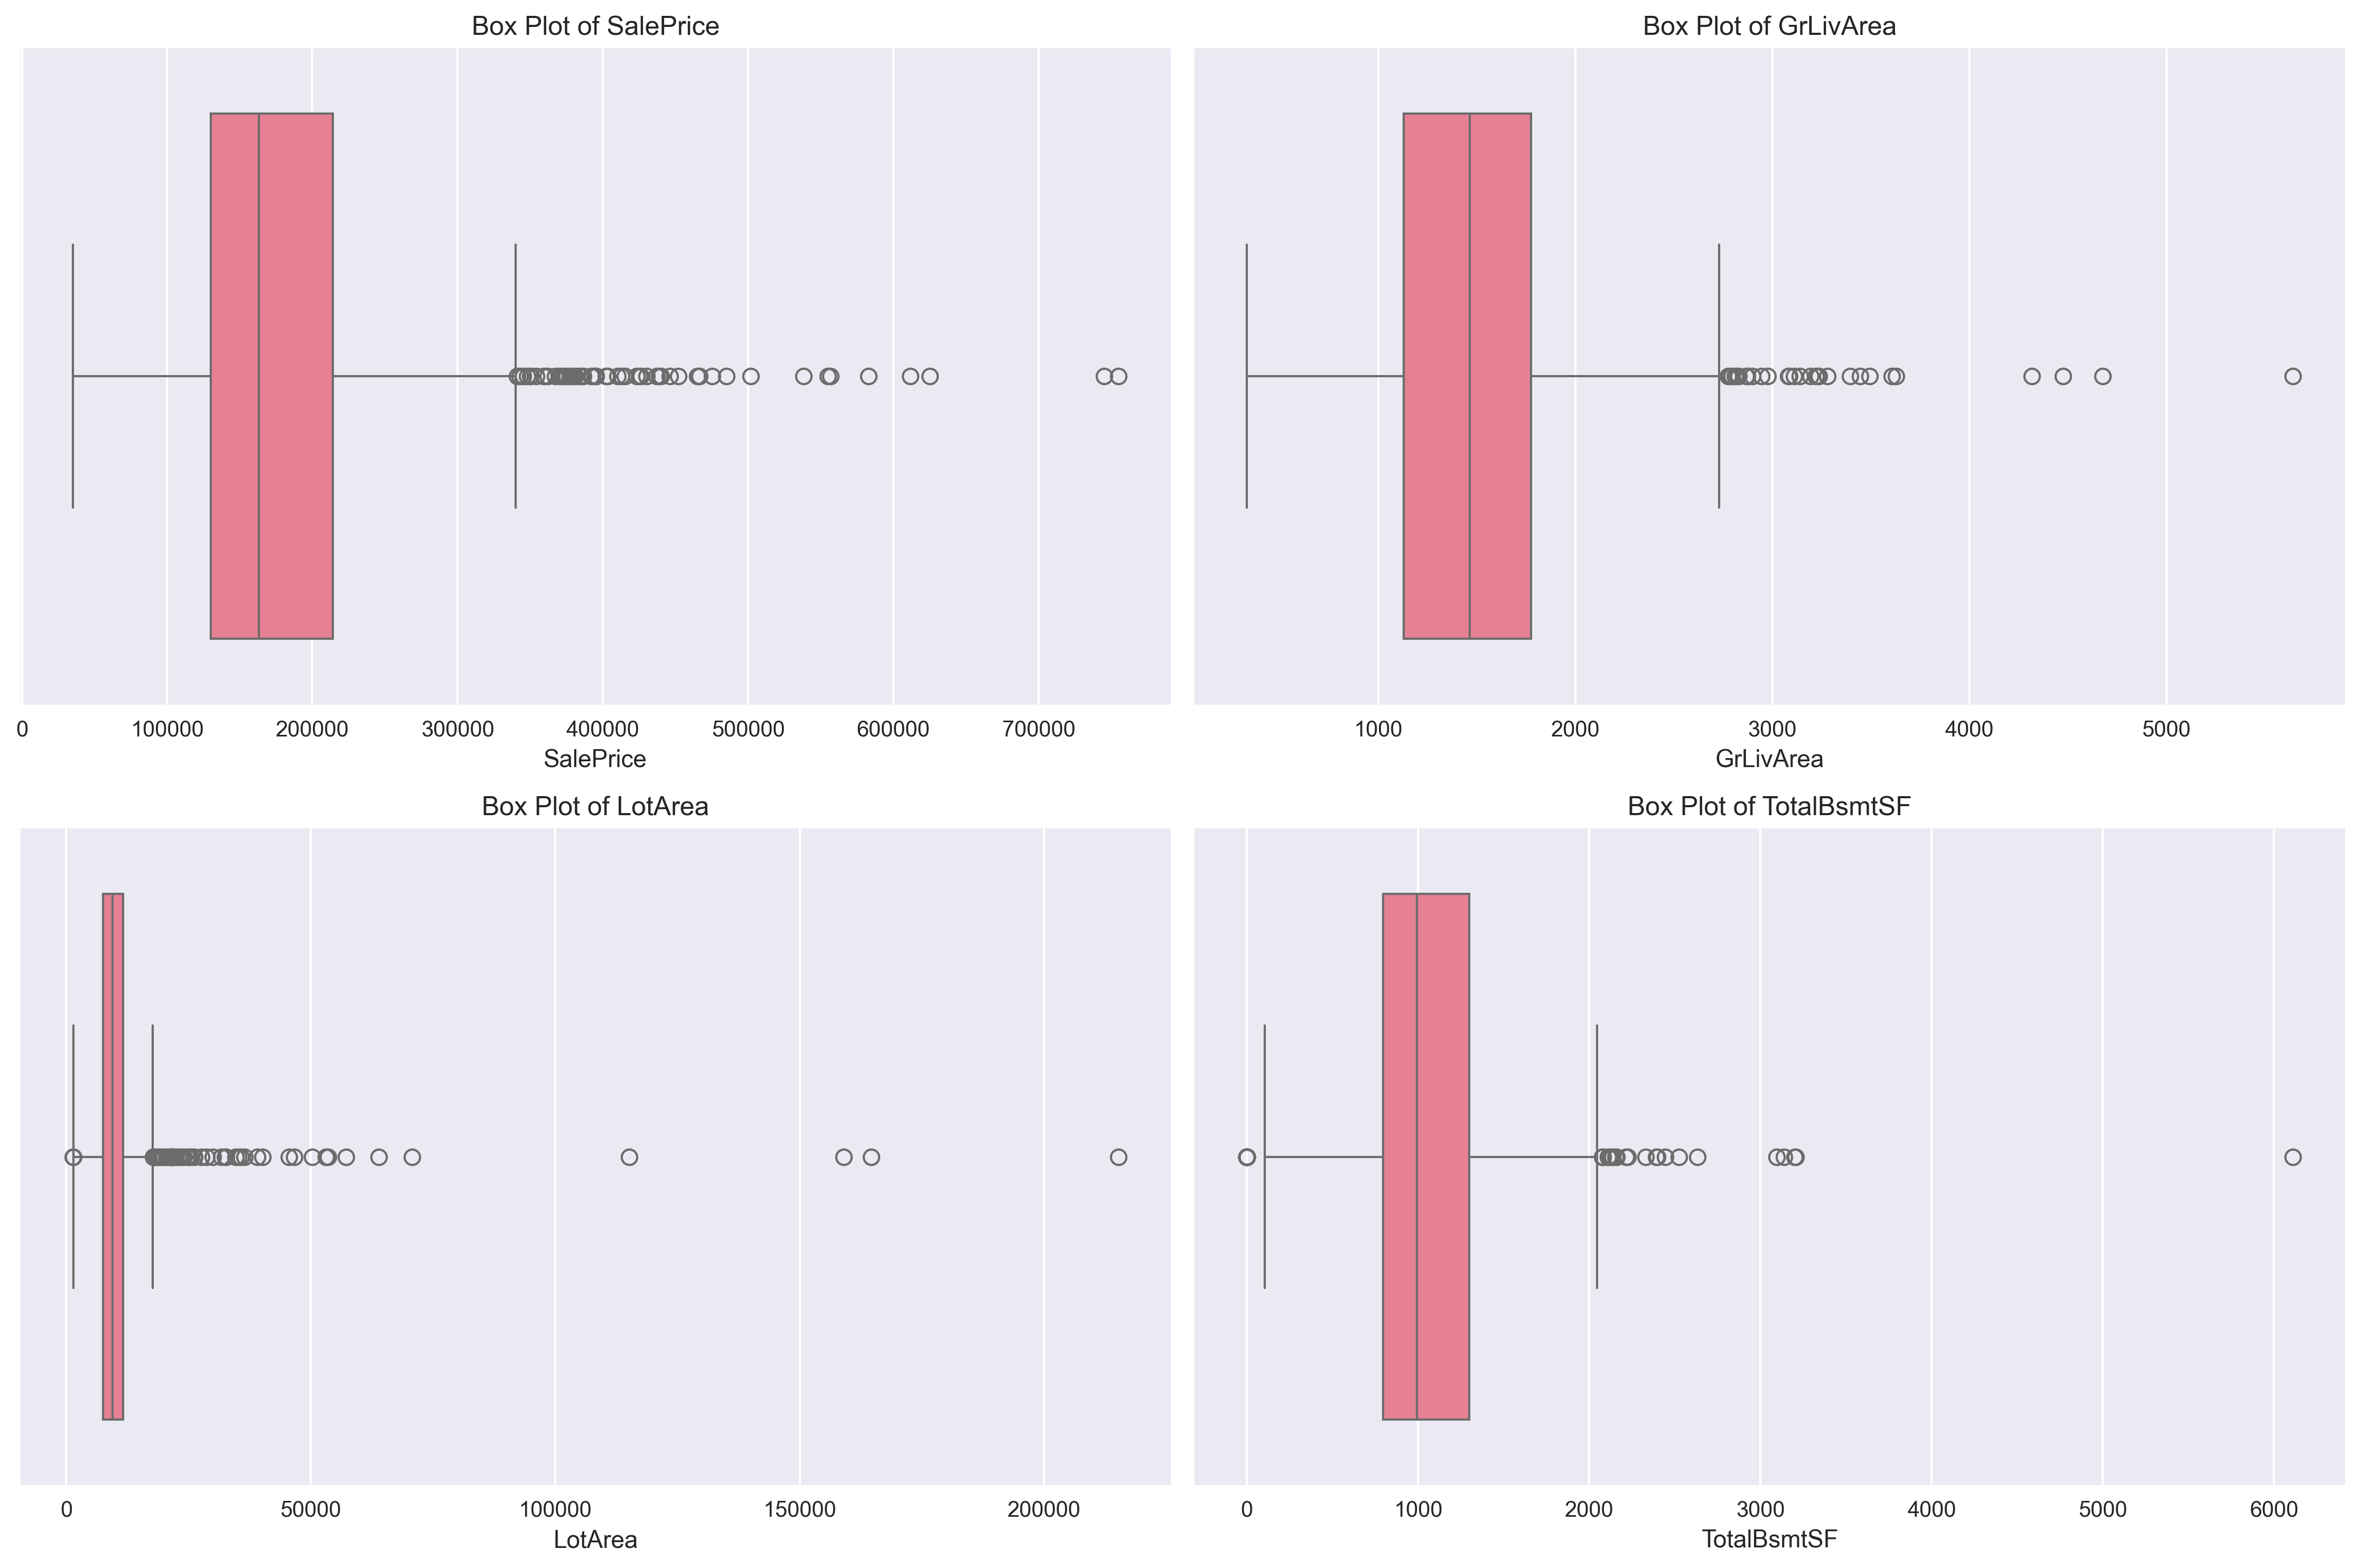
\includegraphics[width=1.0\textwidth]{figures/outliers_boxplot.png}
    \caption{Boxplots Showing Outliers in Key Features}
    \label{fig:outliers}
\end{figure}

Outlier detection reveals:
\begin{itemize}
    \item Several properties with extremely high sale prices (>2.5 IQR)
    \item GrLivArea has notable outliers above 4,000 sq ft
    \item Lot Area shows extreme outliers, with some lots significantly larger than typical
    \item Total Basement SF outliers align with larger homes
\end{itemize}

\section{Feature Importance}
\begin{figure}[H]
    \centering
    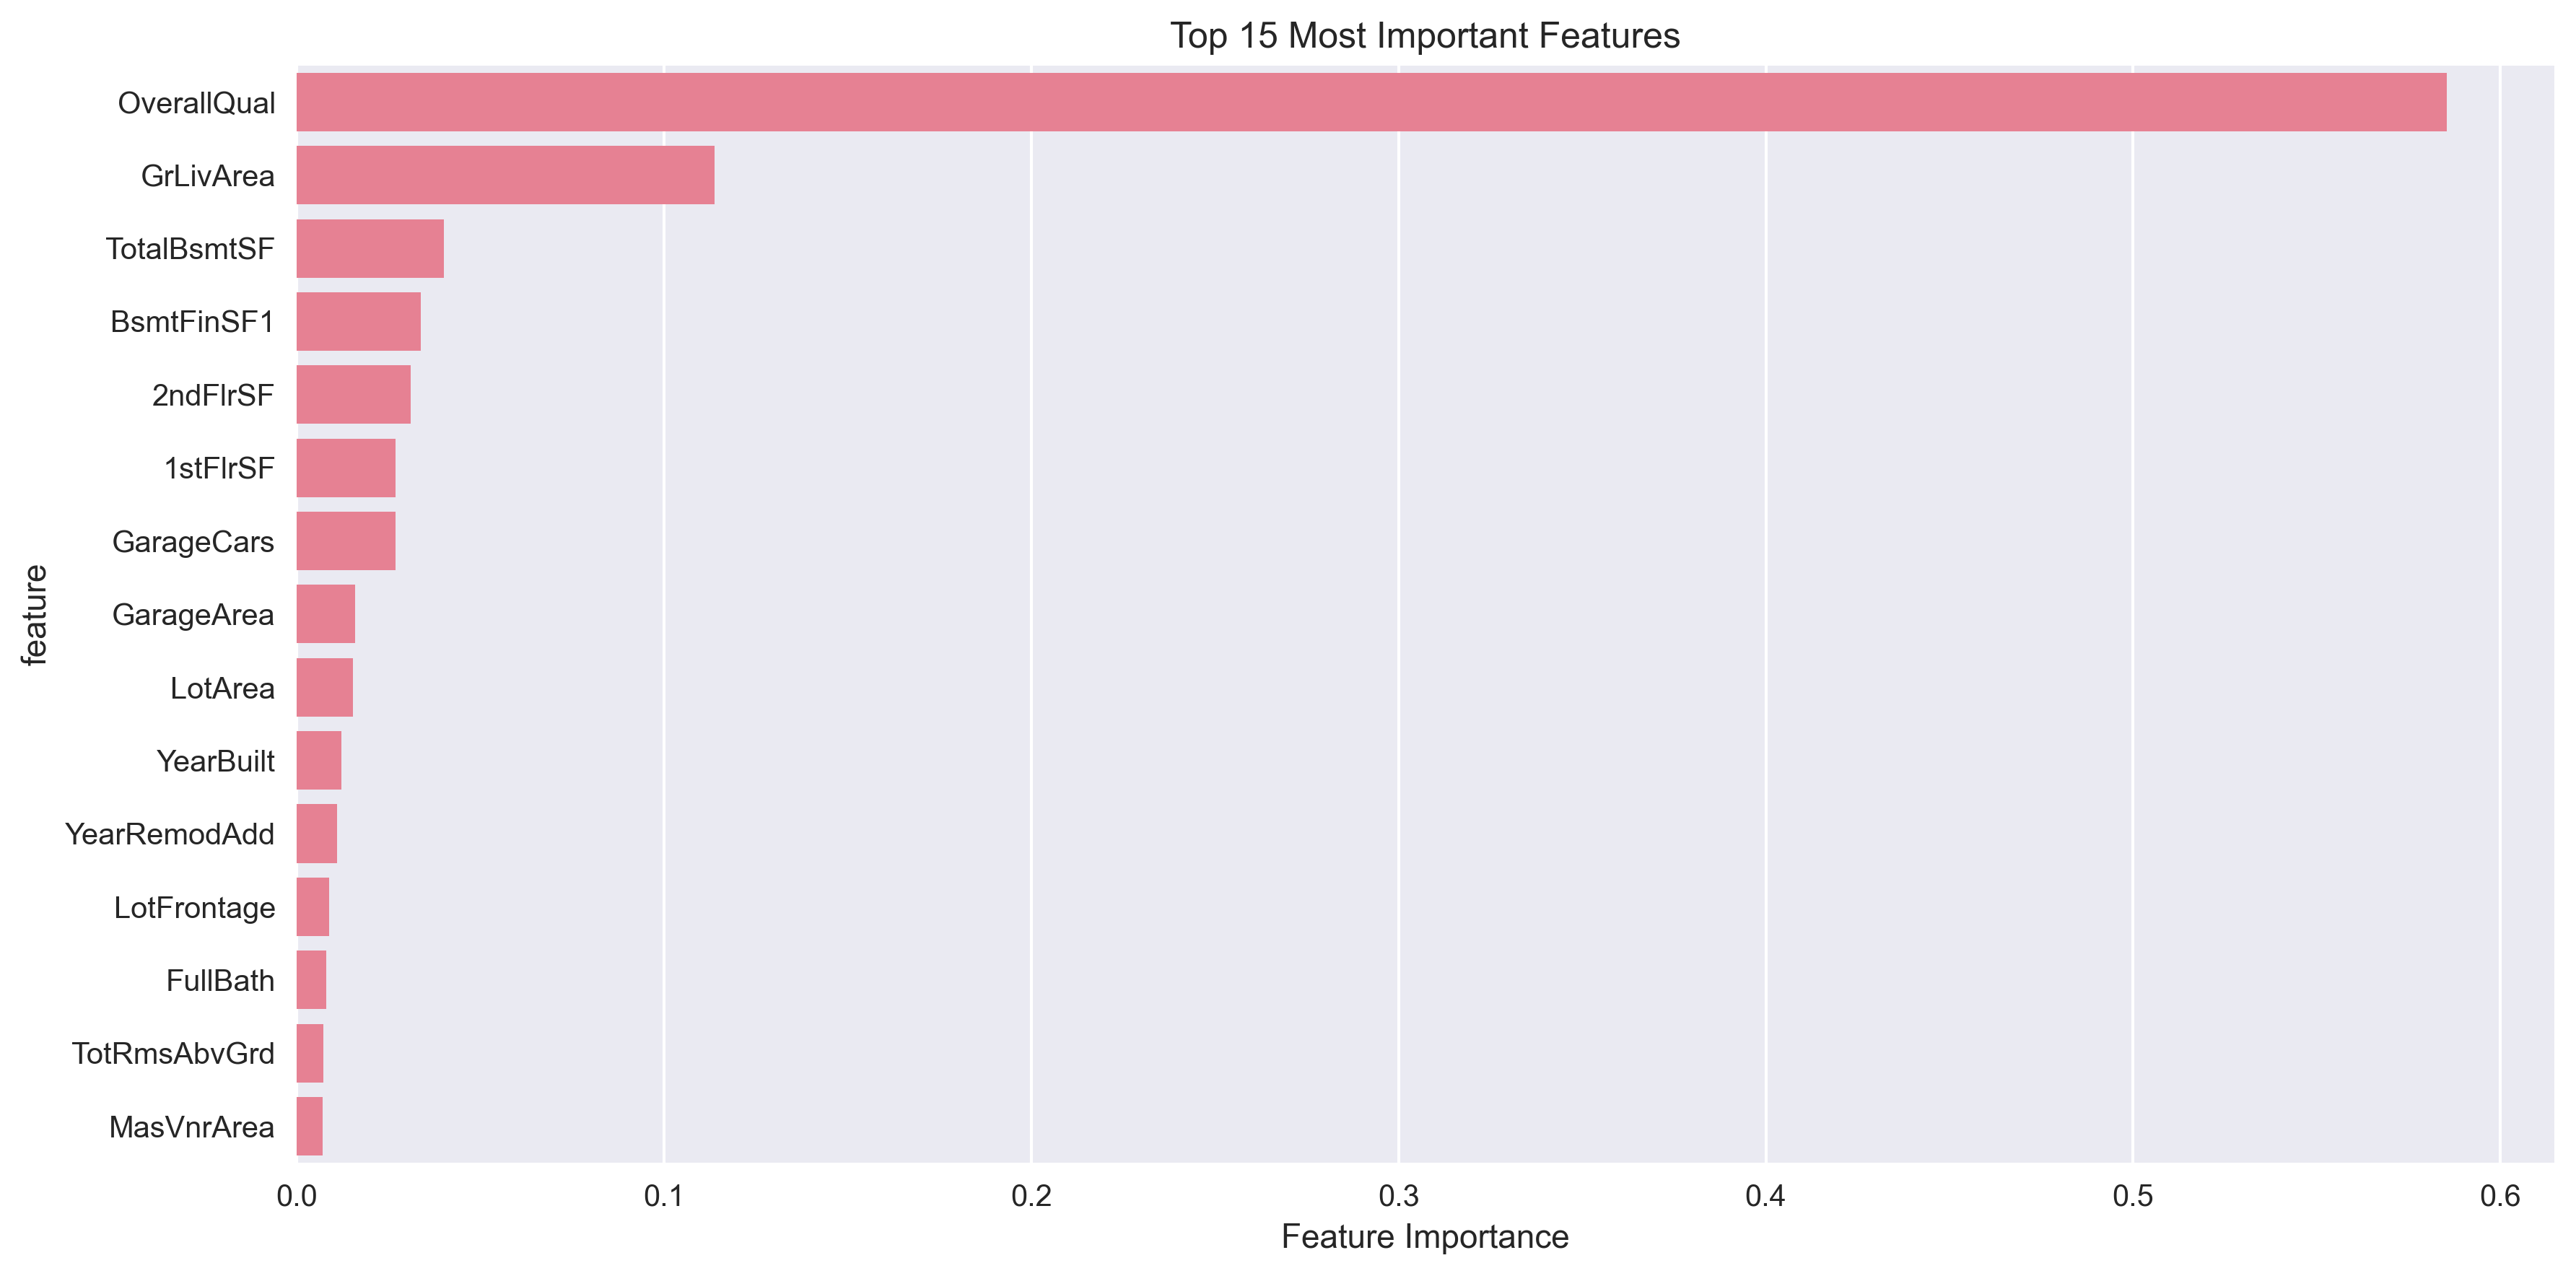
\includegraphics[width=1.0\textwidth]{figures/feature_importance.png}
    \caption{Random Forest Feature Importance Analysis}
    \label{fig:feature_importance}
\end{figure}

The Random Forest analysis identifies key predictors:
\begin{itemize}
    \item Overall Quality emerges as the most important feature
    \item Ground Living Area is the second most important predictor
    \item Year Built and Total Basement SF show significant importance
    \item Garage Area and First Floor SF also contribute meaningfully
\end{itemize}

\section{Key Findings and Recommendations}
Based on the comprehensive EDA, we recommend:
\begin{itemize}
    \item Log transformation of Sale Price and some size-related features
    \item Careful handling of outliers, especially in GrLivArea and Lot Area
    \item Feature engineering combining quality ratings
    \item Neighborhood-based feature engineering
    \item Treatment of missing values based on domain context
    \item Consideration of interaction terms between quality and size features
\end{itemize}

These insights will guide our modeling approach, particularly in:
\begin{itemize}
    \item Feature selection and engineering
    \item Choice of regression techniques
    \item Handling of non-linear relationships
    \item Treatment of categorical variables
\end{itemize}